\documentclass[main.tex]{subfiles}
\begin{document}\newpage
\setdoublesep{0.35700 em}  % 'Bond Spacing'
\setatomsep{1.78500 em}    % 'Fixed Length'
\setbondoffset{0.18265 em} % 'Margin Width'
\newcommand{\bondwidth}{0.06642 em} % 'Line Width'
\setbondstyle{line width = \bondwidth}
\newgeometry{left=0.8in,right=0.8in, top=2.5cm,bottom=2cm}
\fancyhfoffset[E,O]{0pt}
\setlength{\columnsep}{30pt}
\begin{conclusion}
\end{conclusion}
\setstretch{0.3}
\begin{multicols*}{2}


{\raggedright\textsc{\textbf{Intermolecular forces }}\par}

\begin{enumerate}

\item What is the strongest Intermolecular force existing between the molecules of \ce{CH3OH}:
\begin{enumerate}[label=(\alph*)]
\begin{multicols*}{2}
\item dispersion forces
\item dipole forces
\item hydrogen bonds
\end{multicols*}\flushright  {\small Ans: (c)}
\end{enumerate}

\item What is the strongest Intermolecular force existing between the molecules of \ce{H2}:
\begin{enumerate}[label=(\alph*)]
\begin{multicols*}{2}
\item dispersion forces
\item dipole forces
\item hydrogen bonds
\end{multicols*}\flushright  {\small Ans: (a)}
\end{enumerate}


\item What is the strongest Intermolecular force existing between the molecules of \ce{CCl4}:
\begin{enumerate}[label=(\alph*)]
\begin{multicols*}{2}
\item dispersion forces
\item dipole forces
\item hydrogen bonds
\end{multicols*}\flushright  {\small Ans: (a)}
\end{enumerate}

\item What is the strongest Intermolecular force existing between the molecules of \ce{CH4}:
\begin{enumerate}[label=(\alph*)]
\begin{multicols*}{2}
\item dispersion forces
\item dipole forces
\item hydrogen bonds
\end{multicols*}\flushright  {\small Ans: (a)}
\end{enumerate}

\item What is the strongest Intermolecular force existing between the molecules of \ce{CCl3H}:
\begin{enumerate}[label=(\alph*)]
\begin{multicols*}{2}
\item dispersion forces
\item dipole forces
\item hydrogen bonds
\end{multicols*}\flushright  {\small Ans: (b)}
\end{enumerate}

\item What is the strongest Intermolecular force existing between the molecules of \ce{HF}:
\begin{enumerate}[label=(\alph*)]
\begin{multicols*}{2}
\item dispersion forces
\item dipole forces
\item hydrogen bonds
\end{multicols*}\flushright  {\small Ans: (c)}
\end{enumerate}


\item What is the strongest Intermolecular force existing between the molecules of \ce{HCl}:
\begin{enumerate}[label=(\alph*)]
\begin{multicols*}{2}
\item dispersion forces
\item dipole forces
\item hydrogen bonds
\end{multicols*}\flushright  {\small Ans: (b)}
\end{enumerate}

\item Which molecule forms intermolecular H bonds?
\begin{enumerate}[label=(\alph*)]
\begin{multicols*}{2}
\item  \ce{HF}
\item  \ce{H2}
\end{multicols*}\flushright  {\small Ans: (a)}
\end{enumerate}

\item Which molecule forms intermolecular H bonds?
\begin{enumerate}[label=(\alph*)]
\begin{multicols*}{2}
\item  \ce{NH3}
\item  \ce{CH4}
\end{multicols*}\flushright  {\small Ans: (a)}
\end{enumerate}


\item Which molecule forms intermolecular H bonds?
\begin{enumerate}[label=(\alph*)]
\begin{multicols*}{2}
\item  \ce{CH3-O-CH3}
\item  \ce{H2O}
\end{multicols*}\flushright  {\small Ans: (b)}
\end{enumerate}

\item Which molecule or ion has stronger dipole forces? 
\begin{enumerate}[label=(\alph*)]
\begin{multicols*}{2}
\item  \ce{HCl}
\item  \ce{HF}
\end{multicols*}\flushright  {\small Ans: (b)}
\end{enumerate}


\item Which molecule or ion has stronger dispersion forces? 
\begin{enumerate}[label=(\alph*)]
\begin{multicols*}{2}
\item  \ce{CH3CH3}
\item  \ce{CH4}
\end{multicols*}\flushright  {\small Ans: (a)}
\end{enumerate}

\item Which substance has higher boiling point? 
\begin{enumerate}[label=(\alph*)]
\begin{multicols*}{2}
\item  \ce{CH3CH3}
\item  \ce{CH4}
\end{multicols*}\flushright  {\small Ans: (a)}
\end{enumerate}

\item Which substance has higher boiling point? 
\begin{enumerate}[label=(\alph*)]
\begin{multicols*}{2}
\item  \ce{CO2}
\item  \ce{H2O}
\end{multicols*}\flushright  {\small Ans: (b)}
\end{enumerate}

{\raggedright\textsc{\textbf{Solid state }}\par}


\item Indicate the number of atoms  contained in the body-centered (bcc) cubic unit cell, for structures with the same type of atoms?
\begin{enumerate}[label=(\alph*)]
\begin{multicols*}{2}
\item  1
\item  2
\item  4
\end{multicols*}\flushright  {\small Ans: (b)}
\end{enumerate}


\item Indicate the number of atoms  contained in the simple cubic (sc) unit cell, for structures with the same type of atoms?
\begin{enumerate}[label=(\alph*)]
\begin{multicols*}{2}
\item  1
\item  2
\item  4
\end{multicols*}\flushright  {\small Ans: (b)}
\end{enumerate}





\item The image displays the structure of Polonium. What is the number of atoms per unit cell for this metal?
\begin{center}
\scalebox{0.2}{
\begin{tikzpicture}
\newcommand\pgfmathsinandcos[3]{%
  \pgfmathsetmacro#1{sin(#3)}%
  \pgfmathsetmacro#2{cos(#3)}%
}
\newcommand\LongitudePlane[3][current plane]{%
  \pgfmathsinandcos\sinEl\cosEl{#2} % elevation
  \pgfmathsinandcos\sint\cost{#3} % azimuth
  \tikzset{#1/.style={cm={\cost,\sint*\sinEl,0,\cosEl,(0,0)}}}
}
\newcommand\LatitudePlane[3][current plane]{%
  \pgfmathsinandcos\sinEl\cosEl{#2} % elevation
  \pgfmathsinandcos\sint\cost{#3} % latitude
  \pgfmathsetmacro\yshift{\cosEl*\sint}
  \tikzset{#1/.style={cm={\cost,0,0,\cost*\sinEl,(0,\yshift)}}}
}

\newcommand\ClipLongitudeCircle[2]{
    \LongitudePlane{\angEl}{#1}
    \pgfmathsetmacro\angVis{atan(sin(#1)*cos(\angEl)/sin(\angEl))}
    \path[save path=\tmppath, current plane] (\angVis:\R) arc (\angVis:\angVis+180:\R); % current plane transformation
    \pgfoonew\patha=new spath(\tmppath)
    \pgfmathsetmacro\angVis{-atan(sin(\angEl)*cos(#1)/sin(#1))}
    \path[save path=\tmppath] (-90+\angVis:\R) arc (-90+\angVis:#2 180-90+\angVis:\R); % no coordinate transform (no current plane)
    \pgfoonew\pathb=new spath(\tmppath)
    \patha.concatenate with lineto(,\pathb)
    \patha.close()
    \patha.use path with tikz(clip)
%   \patha.use path with tikz(fill=magenta, opacity=.2)
%   \patha.use path with tikz(draw=magenta, very thick)
}

\newcommand\ClipLatitudeCircle[2]{
    \LatitudePlane{\angEl}{#1}
    \path[save path=\tmppath,current plane] (-180:\R) arc (-180:0:\R);
    \pgfoonew\patha=new spath(\tmppath)
    \path[save path=\tmppath] (0:\R) arc (0:#2 180:\R);
    \pgfoonew\pathb=new spath(\tmppath)
    \patha.concatenate with lineto(,\pathb)
    \patha.close()
    \patha.use path with tikz(clip)
%   \patha.use path with tikz(fill=cyan, opacity=.2)
%   \patha.use path with tikz(draw=cyan, very thick)
}
    \def\COLOR{red}
\newcommand\ClippedEightSphere[4]{
\begin{scope}[transform canvas={shift=(#4)}]
    \ClipLongitudeCircle{45-\angPh}{#1}
    \ClipLongitudeCircle{135-\angPh}{#2}
    \ClipLatitudeCircle{0}{#3}
    \fill[ball color=\COLOR, opacity=0.8] (0,0) circle (\R);
\end{scope}}

\newcommand\ClippedLatitudeSphere[3]{
\begin{scope}[transform canvas={shift=(#1)}]
    \LatitudePlane{\angEl}{#2}
    \ClipLatitudeCircle{0}{#3}
    \fill[ball color=\COLOR, opacity=0.8] (0,0) circle [radius=\R];
\end{scope}}

\newcommand\ClippedLongitudeSphere[3]{
\begin{scope}[transform canvas={shift=(#1)}]
    \LongitudePlane{\angEl}{#2}
    \ClipLongitudeCircle{#2}{#3}
    \fill[ball color=\COLOR, opacity=0.8] (0,0) circle [radius=\R];
\end{scope}}

\newcommand\DrawLongitudeArc[4]{
    \LongitudePlane{\angEl}{#2}
    \begin{scope}[current plane, transform canvas={shift=(#1)}]
    \fill [red] (0,0) -- ++(#3:\R) arc [start angle=#3, delta angle=#4, radius=\R] -- cycle;
    \draw ++(#3:\R) arc [start angle=#3, delta angle=#4, radius=\R];
    \end{scope}}

\newcommand\DrawLatitudeArc[4]{
    \LatitudePlane{\angEl}{#2}
    \begin{scope}[current plane, transform canvas={shift=(#1)}]
    \fill [red] (0,0) -- ++(#3:\R) arc [start angle=#3, delta angle=#4, radius=\R] -- cycle;
    \draw ++(#3:\R) arc [start angle=#3, delta angle=#4, radius=\R];
    \end{scope}}



    \def\D{8} % cubic side length
   \pgfmathsetmacro\R{\D/2} % sphere radius
%    \pgfmathsetmacro\R{sqrt(2)/4*\D} % sphere radius
%   \pgfmathsetmacro\R{sqrt(3)/4*\D} % sphere radius
    \def\angEl{20} % elevation angle in interval [1,89]
    \def\angPh{10} % phase angle in interval [-44,44]
    \pgfmathsetmacro\uofx{cos(-135-\angPh)}
    \pgfmathsetmacro\vofx{sin(-135-\angPh)*sin(\angEl)}
    \pgfmathsetmacro\uofy{cos(-45-\angPh)}
    \pgfmathsetmacro\vofy{sin(-45-\angPh)*sin(\angEl)}
    \pgfmathsetmacro\uofz{0}
    \pgfmathsetmacro\vofz{cos(\angEl)}

    % The coordinates of the cube
    \begin{scope}[x={(\uofx cm,\vofx cm)}, y={(\uofy cm,\vofy cm)}, z={(\uofz cm,\vofz cm)}]
    \coordinate (C1) at (\D,0,0);
    \coordinate (C2) at (\D,0,\D);
    \coordinate (C3) at (0,0,\D);
    \coordinate (C4) at (0,\D,\D);
    \coordinate (C5) at (0,\D,0);
    \coordinate (C6) at (\D,\D,0);
    \coordinate (C7) at (0,0,0);
    \coordinate (C8) at (\D,\D,\D);
%    \foreach \n in {1,2,...,8} \node at (C\n) {C\n};

    \coordinate (C0) at ($(C2)!.5!(C5)$);
    \coordinate (S1) at ($(C2)!.5!(C6)$);
    \coordinate (S2) at ($(C2)!.5!(C4)$);
    \coordinate (S3) at ($(C8)!.5!(C5)$);
    \coordinate (S4) at ($(C6)!.5!(C7)$);
    \coordinate (S5) at ($(C1)!.5!(C3)$);
    \coordinate (S6) at ($(C5)!.5!(C3)$);
    \end{scope}

    % Draw the clipped spheres
    \ClippedEightSphere{+}{-}{+}{C7}
    \ClippedLongitudeSphere{S5}{45-\angPh}{+}
    \ClippedLongitudeSphere{S6}{135-\angPh}{-}
    \ClippedLatitudeSphere{S4}{0}{+}

    \ClippedEightSphere{-}{+}{-}{C8}
    \ClippedEightSphere{+}{-}{-}{C3}
    \ClippedEightSphere{+}{+}{-}{C2}
 %  \fill[ball color=white] (C0) circle [radius=\R];
    \ClippedEightSphere{-}{-}{-}{C4}
    \ClippedEightSphere{+}{+}{+}{C1}
    \ClippedEightSphere{-}{-}{+}{C5}
    \ClippedEightSphere{-}{+}{+}{C6}

%    % Draw the half spheres
%    \ClippedLatitudeSphere{S2}{0}{-}
%    \ClippedLongitudeSphere{S3}{45-\angPh}{-}
%    \ClippedLongitudeSphere{S1}{135-\angPh}{+}
%    \DrawLatitudeArc{S2}{0}{0}{360}
%    \DrawLongitudeArc{S1}{135-\angPh}{0}{360}
%    \DrawLongitudeArc{S3}{45-\angPh}{0}{360}

    % Draw the Arcs
    \DrawLongitudeArc{C1}{135-\angPh}{90}{90}
    \DrawLongitudeArc{C2}{135-\angPh}{-90}{-90}
    \DrawLongitudeArc{C4}{45-\angPh}{-90}{-90}
    \DrawLongitudeArc{C5}{45-\angPh}{90}{90}
    \DrawLongitudeArc{C6}{135-\angPh}{90}{-90}
    \DrawLongitudeArc{C6}{45-\angPh}{90}{-90}
    \DrawLongitudeArc{C8}{135-\angPh}{-90}{90}
    \DrawLongitudeArc{C8}{45-\angPh}{-90}{90}
    \DrawLatitudeArc{C2}{0}{45-\angPh}{-90}
    \DrawLatitudeArc{C3}{0}{-45-\angPh}{-90}
    \DrawLatitudeArc{C4}{0}{135-\angPh}{90}
    \DrawLatitudeArc{C8}{0}{135-\angPh}{-90}

    % Draw the cube
    \draw (C1)--(C2)--(C3)--(C4)--(C5)--(C6)--cycle;
    \draw (C2)--(C8)--(C6);
    \draw (C8)--(C4);



\end{tikzpicture}
}
\end{center}
\begin{flushright}\small Ans: 1\end{flushright}

\item The image displays the structure of Gold. What is the number of atoms per unit cell for this metal?
\begin{center}
\scalebox{0.2}{
\begin{tikzpicture}
\newcommand\pgfmathsinandcos[3]{%
  \pgfmathsetmacro#1{sin(#3)}%
  \pgfmathsetmacro#2{cos(#3)}%
}
\newcommand\LongitudePlane[3][current plane]{%
  \pgfmathsinandcos\sinEl\cosEl{#2} % elevation
  \pgfmathsinandcos\sint\cost{#3} % azimuth
  \tikzset{#1/.style={cm={\cost,\sint*\sinEl,0,\cosEl,(0,0)}}}
}
\newcommand\LatitudePlane[3][current plane]{%
  \pgfmathsinandcos\sinEl\cosEl{#2} % elevation
  \pgfmathsinandcos\sint\cost{#3} % latitude
  \pgfmathsetmacro\yshift{\cosEl*\sint}
  \tikzset{#1/.style={cm={\cost,0,0,\cost*\sinEl,(0,\yshift)}}}
}

\newcommand\ClipLongitudeCircle[2]{
    \LongitudePlane{\angEl}{#1}
    \pgfmathsetmacro\angVis{atan(sin(#1)*cos(\angEl)/sin(\angEl))}
    \path[save path=\tmppath, current plane] (\angVis:\R) arc (\angVis:\angVis+180:\R); % current plane transformation
    \pgfoonew\patha=new spath(\tmppath)
    \pgfmathsetmacro\angVis{-atan(sin(\angEl)*cos(#1)/sin(#1))}
    \path[save path=\tmppath] (-90+\angVis:\R) arc (-90+\angVis:#2 180-90+\angVis:\R); % no coordinate transform (no current plane)
    \pgfoonew\pathb=new spath(\tmppath)
    \patha.concatenate with lineto(,\pathb)
    \patha.close()
    \patha.use path with tikz(clip)
%   \patha.use path with tikz(fill=magenta, opacity=.2)
%   \patha.use path with tikz(draw=magenta, very thick)
}

\newcommand\ClipLatitudeCircle[2]{
    \LatitudePlane{\angEl}{#1}
    \path[save path=\tmppath,current plane] (-180:\R) arc (-180:0:\R);
    \pgfoonew\patha=new spath(\tmppath)
    \path[save path=\tmppath] (0:\R) arc (0:#2 180:\R);
    \pgfoonew\pathb=new spath(\tmppath)
    \patha.concatenate with lineto(,\pathb)
    \patha.close()
    \patha.use path with tikz(clip)
%   \patha.use path with tikz(fill=cyan, opacity=.2)
%   \patha.use path with tikz(draw=cyan, very thick)
}
    \def\COLOR{yellow}
\newcommand\ClippedEightSphere[4]{
\begin{scope}[transform canvas={shift=(#4)}]
    \ClipLongitudeCircle{45-\angPh}{#1}
    \ClipLongitudeCircle{135-\angPh}{#2}
    \ClipLatitudeCircle{0}{#3}
    \fill[ball color=\COLOR, opacity=0.8] (0,0) circle (\R);
\end{scope}}

\newcommand\ClippedLatitudeSphere[3]{
\begin{scope}[transform canvas={shift=(#1)}]
    \LatitudePlane{\angEl}{#2}
    \ClipLatitudeCircle{0}{#3}
    \fill[ball color=\COLOR, opacity=0.8] (0,0) circle [radius=\R];
\end{scope}}

\newcommand\ClippedLongitudeSphere[3]{
\begin{scope}[transform canvas={shift=(#1)}]
    \LongitudePlane{\angEl}{#2}
    \ClipLongitudeCircle{#2}{#3}
    \fill[ball color=\COLOR, opacity=0.8] (0,0) circle [radius=\R];
\end{scope}}

\newcommand\DrawLongitudeArc[4]{
    \LongitudePlane{\angEl}{#2}
    \begin{scope}[current plane, transform canvas={shift=(#1)}]
    \fill [\COLOR] (0,0) -- ++(#3:\R) arc [start angle=#3, delta angle=#4, radius=\R] -- cycle;
    \draw ++(#3:\R) arc [start angle=#3, delta angle=#4, radius=\R];
    \end{scope}}

\newcommand\DrawLatitudeArc[4]{
    \LatitudePlane{\angEl}{#2}
    \begin{scope}[current plane, transform canvas={shift=(#1)}]
    \fill [\COLOR] (0,0) -- ++(#3:\R) arc [start angle=#3, delta angle=#4, radius=\R] -- cycle;
    \draw ++(#3:\R) arc [start angle=#3, delta angle=#4, radius=\R];
    \end{scope}}



    \def\D{8} % cubic side length
%   \pgfmathsetmacro\R{\D/2} % sphere radius
    \pgfmathsetmacro\R{sqrt(2)/4*\D} % sphere radius
 %  \pgfmathsetmacro\R{sqrt(3)/4*\D} % sphere radius
    \def\angEl{20} % elevation angle in interval [1,89]
    \def\angPh{10} % phase angle in interval [-44,44]
    \pgfmathsetmacro\uofx{cos(-135-\angPh)}
    \pgfmathsetmacro\vofx{sin(-135-\angPh)*sin(\angEl)}
    \pgfmathsetmacro\uofy{cos(-45-\angPh)}
    \pgfmathsetmacro\vofy{sin(-45-\angPh)*sin(\angEl)}
    \pgfmathsetmacro\uofz{0}
    \pgfmathsetmacro\vofz{cos(\angEl)}

    % The coordinates of the cube
    \begin{scope}[x={(\uofx cm,\vofx cm)}, y={(\uofy cm,\vofy cm)}, z={(\uofz cm,\vofz cm)}]
    \coordinate (C1) at (\D,0,0);
    \coordinate (C2) at (\D,0,\D);
    \coordinate (C3) at (0,0,\D);
    \coordinate (C4) at (0,\D,\D);
    \coordinate (C5) at (0,\D,0);
    \coordinate (C6) at (\D,\D,0);
    \coordinate (C7) at (0,0,0);
    \coordinate (C8) at (\D,\D,\D);
%    \foreach \n in {1,2,...,8} \node at (C\n) {C\n};

    \coordinate (C0) at ($(C2)!.5!(C5)$);
    \coordinate (S1) at ($(C2)!.5!(C6)$);
    \coordinate (S2) at ($(C2)!.5!(C4)$);
    \coordinate (S3) at ($(C8)!.5!(C5)$);
    \coordinate (S4) at ($(C6)!.5!(C7)$);
    \coordinate (S5) at ($(C1)!.5!(C3)$);
    \coordinate (S6) at ($(C5)!.5!(C3)$);
    \end{scope}

    % Draw the clipped spheres
    \ClippedEightSphere{+}{-}{+}{C7}
    \ClippedLongitudeSphere{S5}{45-\angPh}{+}
    \ClippedLongitudeSphere{S6}{135-\angPh}{-}
    \ClippedLatitudeSphere{S4}{0}{+}

    \ClippedEightSphere{-}{+}{-}{C8}
    \ClippedEightSphere{+}{-}{-}{C3}
    \ClippedEightSphere{+}{+}{-}{C2}
%   \fill[ball color=white] (C0) circle [radius=\R];
    \ClippedEightSphere{-}{-}{-}{C4}
    \ClippedEightSphere{+}{+}{+}{C1}
    \ClippedEightSphere{-}{-}{+}{C5}
    \ClippedEightSphere{-}{+}{+}{C6}

%    % Draw the half spheres
    \ClippedLatitudeSphere{S2}{0}{-}
    \ClippedLongitudeSphere{S3}{45-\angPh}{-}
    \ClippedLongitudeSphere{S1}{135-\angPh}{+}
    \DrawLatitudeArc{S2}{0}{0}{360}
    \DrawLongitudeArc{S1}{135-\angPh}{0}{360}
    \DrawLongitudeArc{S3}{45-\angPh}{0}{360}

    % Draw the Arcs
    \DrawLongitudeArc{C1}{135-\angPh}{90}{90}
    \DrawLongitudeArc{C2}{135-\angPh}{-90}{-90}
    \DrawLongitudeArc{C4}{45-\angPh}{-90}{-90}
    \DrawLongitudeArc{C5}{45-\angPh}{90}{90}
    \DrawLongitudeArc{C6}{135-\angPh}{90}{-90}
    \DrawLongitudeArc{C6}{45-\angPh}{90}{-90}
    \DrawLongitudeArc{C8}{135-\angPh}{-90}{90}
    \DrawLongitudeArc{C8}{45-\angPh}{-90}{90}
    \DrawLatitudeArc{C2}{0}{45-\angPh}{-90}
    \DrawLatitudeArc{C3}{0}{-45-\angPh}{-90}
    \DrawLatitudeArc{C4}{0}{135-\angPh}{90}
    \DrawLatitudeArc{C8}{0}{135-\angPh}{-90}

    % Draw the cube
    \draw (C1)--(C2)--(C3)--(C4)--(C5)--(C6)--cycle;
    \draw (C2)--(C8)--(C6);
    \draw (C8)--(C4);



\end{tikzpicture}
}
\end{center}
\begin{flushright}\small Ans: 4\end{flushright}


\item Classify the following crystalline solid: cesium chloride.
\begin{enumerate}[label=(\alph*)]
\begin{multicols*}{2}
\item  atomic solid
\item  molecular solid
\item  ionic solid
\end{multicols*}\flushright  {\small Ans: (c)}
\end{enumerate}



\item Classify the following crystalline solid: tungsten.
\begin{enumerate}[label=(\alph*)]
\begin{multicols*}{2}
\item  atomic solid
\item  molecular solid
\item  ionic solid
\end{multicols*}\flushright  {\small Ans: (a)}
\end{enumerate}

\item Classify the following crystalline solid: acetic acid.
\begin{enumerate}[label=(\alph*)]
\begin{multicols*}{2}
\item  atomic solid
\item  molecular solid
\item  ionic solid
\end{multicols*}\flushright  {\small Ans: (b)}
\end{enumerate}

\item Classify the following crystalline solid: hydrogen sulfide.
\begin{enumerate}[label=(\alph*)]
\begin{multicols*}{2}
\item  atomic solid
\item  molecular solid
\item  ionic solid
\end{multicols*}\flushright  {\small Ans: (b)}
\end{enumerate}


\item An element crystallizes in a face-centered cubic lattice and has a density of 1.5 $g\cdot mL^{-1}$ and a cell parameter of $452$pm. Calculate the approximate mass of the element.

\begin{flushright}\small Ans: 20 $g\cdot mol^{-1}$\end{flushright}


\item Calculate the formula for the following unit cell:
\begin{center}
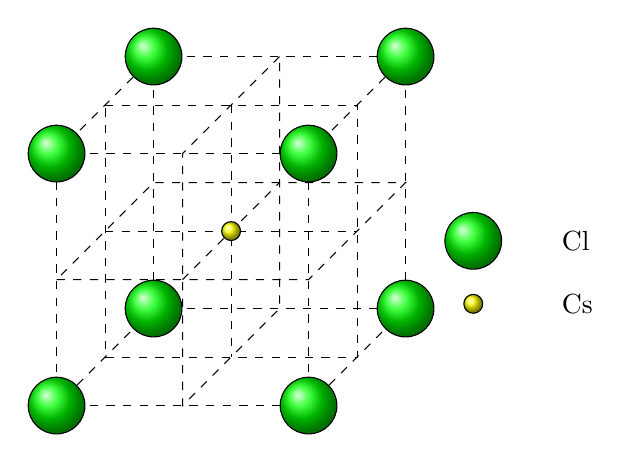
\begin{tikzpicture}[scale = 0.8]
%points on cube
\coordinate (A) at (0,0,0);
\coordinate (B) at (0,0,4);
\coordinate (D) at (0,4,0);
\coordinate (C) at (0,4,4);
\coordinate (E) at (4,0,0);
\coordinate (F) at (4,0,4);
\coordinate (H) at (4,4,0);
\coordinate (G) at (4,4,4);
%center of faces
\coordinate (I) at (0,2,2); %center of face ABCD
\coordinate (J) at (4,2,2); %center of face EFGH
\coordinate (K) at (2,4,2); %center of face DCGH
\coordinate (L) at (2,0,2); %center of face ABFE
\coordinate (M) at (2,2,4); %center of face CBGF
\coordinate (N) at (2,2,0); %center of face DAEH
%connectors
\coordinate (O) at (1,1,3);
\coordinate (P) at (1,3,1);
\coordinate (Q) at (3,1,1);
\coordinate (R) at (3,3,3);
%draw cube
\draw [dashed] (A) -- (B);
\draw [dashed] (B) -- (C);
\draw [dashed] (C) -- (D);
\draw [dashed] (D) -- (A);
\draw [dashed] (E) -- (F);
\draw [dashed] (F) -- (G);
\draw [dashed] (G) -- (H);
\draw [dashed] (H) -- (E);
\draw [dashed] (A) -- (E);
\draw [dashed] (B) -- (F);
\draw [dashed] (C) -- (G);
\draw [dashed] (D) -- (H);
%\draw [dashed] (2,2,2) -- (A);\draw [dashed] (2,2,2) -- (B);\draw [dashed] (2,2,2) -- (C);\draw [dashed] (2,2,2) -- (D);\draw [dashed] (2,2,2) -- (E);\draw [dashed] (2,2,2) -- (F);\draw [dashed] (2,2,2) -- (G);
\draw [dashed] (0,4,2) -- (4,4,2) -- (4,0,2)-- (0,0,2) -- cycle;
\draw [dashed] (2,4,0) -- (2,4,4) -- (2,0,4)-- (2,0,0) -- cycle;
\draw [dashed] (0,2,4)  -- (4,2,4) -- (4,2,0)  -- (0,2,0) -- cycle;
\draw [dashed] (I)  -- (J) ;
\draw [dashed] (K)  -- (L) ;
\draw [dashed] (M)  -- (N) ;
%Holes 
\coordinate (A1) at (0,4,2);
\coordinate (A2) at (4,4,2);
\coordinate (A3) at (4,0,2);
\coordinate (A4) at (0,0,2);
\coordinate (A5) at (2,4,0);
\coordinate (A6) at  (2,4,4);
\coordinate (A7) at (2,0,4);
\coordinate (A8) at (2,0,0);
\coordinate (A9) at (0,2,4);
\coordinate (A10) at (4,2,4);
\coordinate (A11) at (4,2,0);
\coordinate (A12) at (0,2,0);
\coordinate (A13) at (2,2,2);
 \def\COLORA{green};
  \def\COLORB{yellow};
%place non-atom cube corners
\shadedraw [ball color= \COLORA] (A) circle (0.45cm);
\shadedraw [ball color= \COLORA] (C) circle (0.45cm);
\shadedraw [ball color= \COLORA] (F) circle (0.45cm);
\shadedraw [ball color= \COLORA] (G) circle (0.45cm);
\shadedraw [ball color= \COLORA] (B) circle (0.45cm);
\shadedraw [ball color=\COLORA] (D) circle (0.45cm);
\shadedraw [ball color= \COLORA] (E) circle (0.45cm);
\shadedraw [ball color= \COLORA] (H) circle (0.45cm);



\shadedraw [ball color= \COLORB] (A13) circle (0.15cm);


\shadedraw [ball color= \COLORB, yshift=-2cm] (7,4,5) circle (0.15cm) node [right, xshift=1cm] {Cs};
\shadedraw [ball color= \COLORA, yshift=-2cm] (7,5,5) circle (0.45cm) node [right, xshift=1cm] {Cl};

%draw the center of each face
\end{tikzpicture}\end{center}

\begin{flushright}\small Ans: \ce{Cs1Cl1}\end{flushright}

{\raggedright\textsc{\textbf{Liquid state }}\par}

\item A liquid has a  enthalpy of vaporization of 30 $kJ/mol$ and a boiling point of
122C$^{\circ}$ at 1.00 atm. Calculate its vapor pressure at 200C$^{\circ}$.
\begin{flushright}\small Ans: 4.51atm\end{flushright}

\item What is the  enthalpy of vaporization of a liquid that has a vapor pressure of
500 torr at 100C$^{\circ}$ and a boiling point of 90C$^{\circ}$ at 460 torr?
\begin{flushright}\small Ans: 9.3 $kJ/mol$\end{flushright}


\restoregeometry
\end{enumerate}
\end{multicols*}
\pagecolor{green!10}\afterpage{\nopagecolor}\newpage
\end{document}
